\documentclass[titlepage,12pt]{article}

\usepackage[utf8]{inputenc}
\usepackage[a4paper, total={6in, 8in},headheight=14pt]{geometry}
\usepackage{newtxtext,newtxmath}
\usepackage[scaled=1]{couriers}
\usepackage[spanish]{babel}
\usepackage{microtype}
\usepackage[bottom]{footmisc}
\usepackage{fancyhdr}
\usepackage{graphicx}
\usepackage{blindtext}
\usepackage{scrextend}
\usepackage{tocloft}
\usepackage{parskip}
\usepackage{multicol}
\usepackage{subcaption}
\usepackage{wrapfig}
\usepackage{multicol}
\usepackage{verbatimbox}
\usepackage[nottoc, notlot, notlof]{tocbibind}
\usepackage{listingsutf8}
\usepackage{url}
\usepackage[square,numbers]{natbib}
\usepackage{adjustbox}
\usepackage[makeroom]{cancel}
\usepackage[hidelinks]{hyperref}
\usepackage[Glenn]{fncychap}
\usepackage{lastpage}
\usepackage{fancyhdr}

\bibliographystyle{unsrtnat}

\pagestyle{fancy}
\fancyhf{}
\fancyhead[R]{\rightmark}
\fancyfoot[C]{\leftmark}
\fancyfoot[R]{\thepage}
\renewcommand{\footrulewidth}{0.6pt}% Line at the footer visible
\addto\captionscatalan{%
  \renewcommand\contentsname{Índice}%
}

\fancypagestyle{plain}{%
  \fancyhf{}%
  \fancyfoot[R]{\thepage}%
  \renewcommand{\headrulewidth}{0pt}% Line at the header invisible
  \renewcommand{\footrulewidth}{0.6pt}% Line at the footer visible
}


\renewcommand{\cftpartleader}{\cftdotfill{\cftdotsep}}%
\renewcommand{\cftsecleader}{\cftdotfill{\cftdotsep}}%
\renewcommand\familydefault{\sfdefault}

\usepackage{tikz}
\usetikzlibrary{shapes.geometric, arrows}

\newcommand{\Lagr}{\mathcal{L}}
\newcommand{\Xagr}{\mathcal{X}}

\setlength{\skip\footins}{1cm}

\makeatletter
% \patchcmd{<cmd>}{<search>}{<replace>}{<success>}{<failure>}
\patchcmd{\@makechapterhead}{\huge}{\large}{}{}% for \chapter
\patchcmd{\@makechapterhead}{\Huge}{\large}{}{}% for \chapter
\patchcmd{\@makeschapterhead}{\Huge}{\large}{}{}% for \chapter*
\makeatother


\begin{document}

\iftrue
\newcommand{\HRule}{\rule{\linewidth}{0.5mm}}

\thispagestyle{empty}

\begin{center}

{\large Universitat Politècnica de Catalunya}

\medskip
{\large Facultat d'Informàtica de Barcelona (FIB)}

\vfill
{\bfseries\Large Bachelor's Degree Project}

\vfill
\centerline{\mbox{
\includegraphics[width=60mm]{media/FIB_UPC.png}}}

\vfill
\vspace{5mm}

{\LARGE Jordi Gil González}

\vspace{15mm}

% Title in English according to the official assignment
{\LARGE\bfseries Analysis of the Path Tracing \\ rendering method on CPU and GPU}

\normalfont \small \sffamily{}

\vfill

Computer Science Department


\vfill

\begin{tabular}{rl}
Bachelor's Degree Project Director: & Chica Calaf, Antoni \\
\noalign{\vspace{2mm}}
Study programme: & Computer Science\\
\noalign{\vspace{2mm}}
Specialization: & Computer Graphics\\
\end{tabular}

\vfill

\large Academic Year 2019/2020

\large \today

\end{center}

\newpage
\tableofcontents*
\fi

\newpage

\section{Introduction} \label{introduction}

Nowadays, the images generated by computers are very present in both a work and entertainment environment. The creation of realistic images through computer programs has become a necessity. Industries like the film or video games need algorithms capable of representing the real world in a virtual one and, whenever possible, in the shortest possible time.

The study about methods that allow rendering realistic images is not new. Between the early and mid 70s, the first papers about the simulation of light and colours over the surface of three-dimensional models began to be published. To understand how these methods work, we have to keep in mind the common representation of 3D models.

To represent a 3D model it uses a ''polygon mesh'', commonly known as a triangle mesh because, the triangle, is the most used polygon. This mesh consists of a set of vertexes connected through edges and creating faces.  For all face, we can define an orthogonal normal vector. In Figure \ref{dolphin} we can appreciate an example of a 3D model represented by a triangle mesh.

\begin{figure}[H]
	\centering
	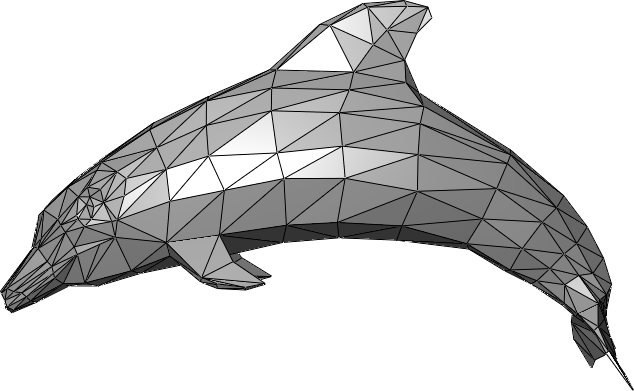
\includegraphics[scale=0.15]{media/Dolphin_triangle_mesh.png}
	\caption{Triangle mesh example. Source: Wikipedia}
	\label{dolphin}
\end{figure}

Returning to lighting calculation methods, the simplest is the \textit{Flat Shading}. To determine the colour of each face of our mesh, this method only takes into account one of all the vertexes that make it up and her normal. In a mesh represented by triangles, it's commonly using the centroid of the triangle. The colour it's interpolated for each vertex. Every face is calculated independently and this produces a visual difference result between continuous faces. In Figure \ref{flat:shading} we can see an object rendered using this method. We might think that adding more vertexes improve the results, but is not the solution because when more vertexes have our meshes, more memory is required and the problem would not be solved. If we zoomed in at the 3D model, we would see the same effect (known as Mach bands) \citep[pp.~5245--5250]{Lotto1999}.

\begin{figure}[H]
	\centering
	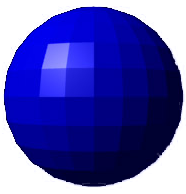
\includegraphics[scale=0.5]{media/Flat-shading-sample.png}
	\caption{Example of \textit{Flat Shading}. Source: Wikipedia}
	\label{flat:shading}
\end{figure}

In the smooth shading methods, the colour change between pixels instead of faces. The result is a smooth transition of colour between adjacent faces.
In 1971 Henri Gouraud presents us in his paper \textit{Continuous Shading of Curved Surfaces} \citep[pp.~623--629]{Henri1971} the Gouraud Shading. With this method, we can add more continuity to the shading, unlike the Flat Shading. The great improvement concerning the method presented above is that it does not require a high-density mesh to simulate greater continuity. For each pixel it's intensity is determined by interpolation of the intensities defined at the vertex of each polygon.

\begin{itemize}
	\item For each vertex, a normal is defined as the average of the normals of the polygons to which said vertex belongs.
	\item Through the using of some lighting model,  e.g. the Phong reflection model, the intensity of each vertex is calculated using the normal taken in the previous point.
	\item For each pixel, the intensity it's interpolated on every vertex to get his intensity.
\end{itemize} 

As we can see in Figure \ref{Gouraud:shading}, the results are notably higher, however, it does not represent the specular highlights. These would be a problem if they appear in the centre of a face.

\begin{figure}[ht]
	\centering
	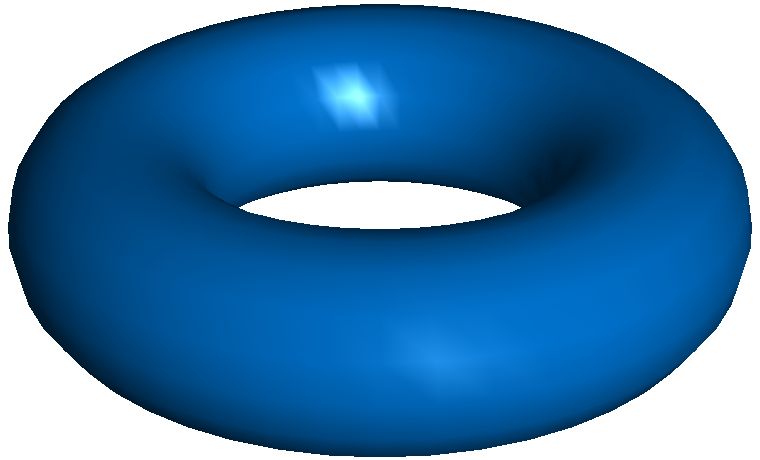
\includegraphics[scale=0.25]{media/Gouraudshading00.png}
	\caption{Ejemplo de \textit{Gouraud Shading}. Source: Wikipedia}
	\label{Gouraud:shading}
\end{figure}

Later, in 1975, Bui Tuong Phong in his PhD thesis \citep[pp.~311--317]{Phong1975} introduces to us the Phong Shading. In the method presented by Phong, instead of calculating the intensity at the vertex, first of all, the normal is defined, interpolated and normalized for each pixel and then using some lighting model the final intensity is determined. Computationally, this method is expensive regarding the others presented, because the calculation is made at fragment (pixel) level.

Phong mention in his paper published by the ACM \citep[p.~311]{Phong1975} that his goal was not to simulate the reality, but rather to add more realism:
\vspace{5mm}

\begin{mdframed}[hidealllines=true,backgroundcolor=gray!20] ''\textit{In trying to improve the quality of the synthetic images, we do not expect to be able to display the object exactly as it would appear in reality, with texture, overcast shadows, etc. We hope only to display an image that approximates the real object closely enough to provide a certain degree of realism.}'' 
\end{mdframed}

Even though these methods represented, as far as realism is concerned, an advance, they do not pretend to simulate reality. Furthermore, these only take into account ambient, diffuse and specular light. They do not take into account the indirect lighting of the scene, an important factor in creating images that produce realistic effects such as reflections.

It was not until the 80s that the first methods capable of rendering realistic images appeared. At the sixth annual conference on \textit{Computer graphics and interactive techniques (SIGGRAPH)}, Turner White presents the Ray Tracing method \citep[pp.~343--349]{Whitted1980}. This method is based on the Ray Casting algorithm, presented by \citep[pp.~37--45]{Appel1968}, consists of trace rays from the observer to all pixels, on for each one, to determine the closest object. Also, once the ray hits on a surface, based on the properties of the materials defined and the light properties, the colour is calculated. In addition, using texture maps we can simulate shadows.

In 1986, David Immel et al. and James T. Kajiya, researchers from Cornell University and California Institute of Technology (Caltech) respectively, at the thirteenth annual conference on \textit{Computer graphics and interactive techniques (SIGGRAPH)} they introduced the \textit{Rendering Equation} \citep[pp.~143--150, pp.~133--142]{Kajiya1986, Immel1986}. This integral equation tries to summarize in one formula how the light interacts with a surface when a ray of light hits her using a bidirectional reflectance distribution function (BRDF). This formula takes into account the number of photons from the source, the incident angle, etcetera.

Exist other methods that can generate realistic images by approximating the RE: Bidirectional Path Tracing, presented by \citep[pp.~145--153]{Lafortune1993}; Photon Mapping, formulated by \citep[pp. ~21--30]{Jensen1996}; Metropolis light Transport, introduced by \citep[pp. ~65--76]{Veach1997}.

\newpage

\section{Contextualization}

During the degree studies, there are several subjects dedicated to computer graphics. In these subjects, we are introduced to realistic rendering methods, but beyond the theoretical introduction to these, they are never put in practice. From here comes the idea of realizing the present project, to be able to go deeper into the subject of realistic rendering and thus create an application based on what has been learned during the studies. Other aspects of computer science seen will also put into practice, such as the creation of parallel applications on both CPUs and GPUs.

As we have pointed out in the last section, rendering true-to-life images is an area of great interests in computer graphics. One of the principal goals is to be able to render images that are indistinguishable from photographs. Following this idea, being able to replicate the behaviour of light in a virtual environment is an important task. It's essential to keep in mind the global illumination of our scene to achieve that realism. The global illumination is compounded by \begin{enumerate*}[label=\roman*)] \item direct illumination \label{item:dl} and \item indirect (global) illumination \label{item:il} \end{enumerate*}. In Figure \ref{globalil}, we can observe a graphic representation of both types of lighting.

\begin{figure}[!ht]
	\centering
	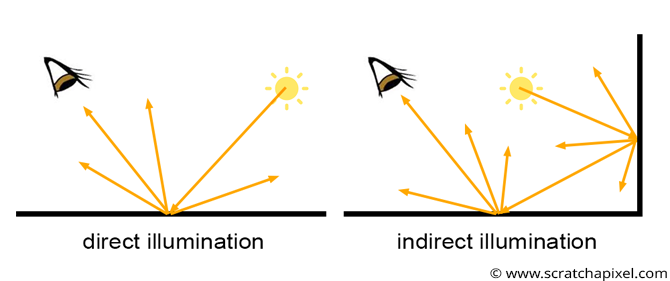
\includegraphics[scale=0.45]{media/shad2-globalillum3.png}
	\caption{Example of \textit{Direct illumination and Indirect illumination}. Source: ScratchPixel}
	\label{globalil}
\end{figure}

\ref{item:dl} Direct illumination is that which strikes a point from the light source.\\
\ref{item:il} Indirect illumination is that which hits one point from the light bouncing off other points in the scene.

Retrieving what was said in the introduction, the first method capable to render realistic images was the Ray Tracing, based on Ray Casting algorithm, a technique that consists in trace rays from the eye or camera to all pixels of an image. The great novelty concerning the algorithm presented by Appel is the recursivity. The Ray Tracing algorithm emits a ray from the virtual camera across the scene to a light source. When a ray hits some surface can produce three new types of rays: \begin{enumerate*}[label=\roman*)] \item
 reflection ray \label{ray:reflected}, \item
 refraction ray and \item
 shadow ray\end{enumerate*}. From this point, a new ray is projected until hits one of the light sources in the scene. When tracing new rays, we can obtain effects like reflections, shadows, caustics, etcetera. If the ray hits a transparent material like glass, the ray is projected through this to simulate the refraction rays. The principal disadvantage is the dependency on the number of polygons in the scene. The more polygons the scene will have, the more inefficient will be the algorithm.

The results obtained are not necessarily photo-realistic despite offering a high degree of realism by being able to accurately treat optical effects such as refraction or reflection. It's mandatory to do some post-processing to be able to simulate effects such as soft shadows or caustics. Rendering photo-realistic images is mandatory approximating the RE. The Path Tracing algorithm, presented by \citep[pp. ~143--150]{Kajiya1986}, is a good example of that.

The Path Tracing algorithm came up as an improvement of the Ray Tracing with the purpose to give a resolution of the rendering equation by the Monte Carlo integration. It is for this reason that the algorithm is inherently able to simulate effects such as motion blur, ambient occlusion and global illumination without any post-processing. Unlike Ray Tracing, in the Path Tracing when a ray is emitted by the virtual camera, this is traced through the scene bouncing in the objects until reaching one light source or sky or run out a limit. The significant difference between the algorithm presented by White is that the algorithm introduced by Kajiya, for each pixel, we keep in mind not only one ray but dozens, hundreds or even thousands. The random sampling is a significant aspect, this means that when a  ray hits a surface, it generates a new ray in a random direction. Once a ray reaches a limit or it is absorbed by a light source, the colour is calculated according to the material properties of the objects it has bounced off. This colour is added to calculate the average between all rays emitted for each pixel. This random sampling produces a noisy result. The more sampling we use, the smoother it becomes.

\begin{figure}[!ht]
	\centering
	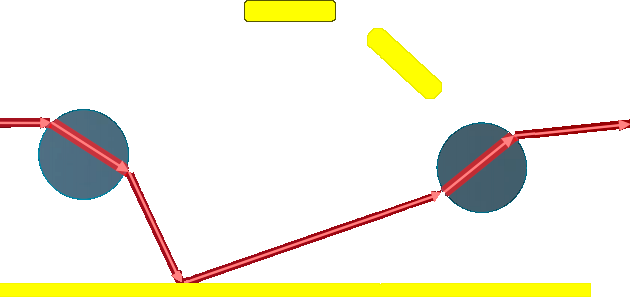
\includegraphics[scale=0.45]{media/lightPathRT.png}
	\caption{Ray Tracing}
	\label{RT_traced}
\end{figure}

\begin{figure}[!ht]
	\centering
	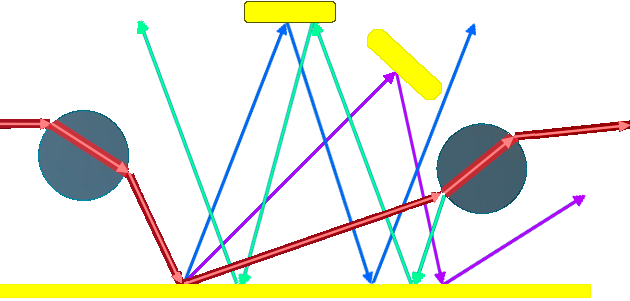
\includegraphics[scale=0.45]{media/lightPathPT.png}
	\caption{Path Tracing}
	\label{PT_traced}
\end{figure}

In Figure \ref{RT_traced} it can be observed what is mentioned in the previous paragraph. In the Ray Tracing, the colour calculation in one pixel depends only from the primary ray and his bounces until reach a light source. However, in Figure 5 it can be observed that for each bounced, multiple rays are traced. This occurs because when a ray hits a diffuse surface, the photons are scattered in all directions. 

The number of polygons in a scene is irrelevant for Path Tracing, the scene complexity does not affect proportionally the algorithm's performance. How we mentioned above, in the first method only one ray is traced for each polygon. However, in Kajiya's method, the ray is traced per pixel. Because each pixel is independent of each other, we can exploit the concurrency provided by CPUs and GPUs.

\begin{figure}[H]
	\centering
	\begin{subfigure}{.3\textwidth}
		\centering
		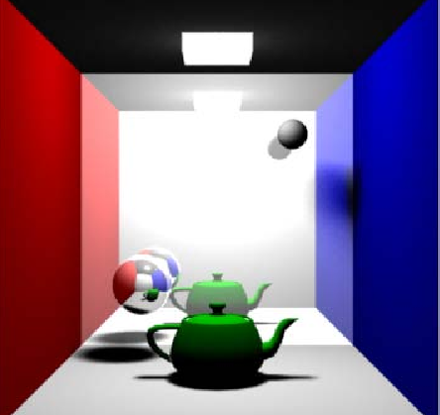
\includegraphics[width=.8\textwidth]{media/RayTracing.png}
		\caption{\textit{Ray Tracing}.}
		\label{RT}
	\end{subfigure}
	\begin{subfigure}{.3\textwidth}
		\centering
		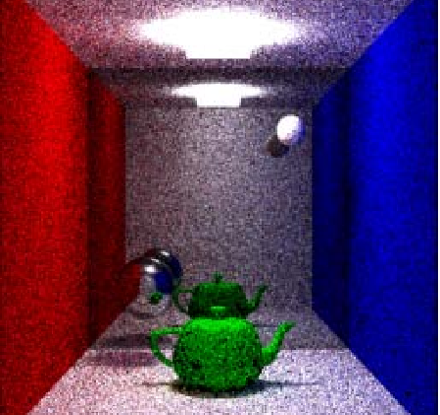
\includegraphics[width=.8\textwidth]{media/PathTracing.png}
		\caption{\textit{Path Tracing} with noise.}
		\label{PTN}
	\end{subfigure}
	\begin{subfigure}{.3\textwidth}
		\centering
		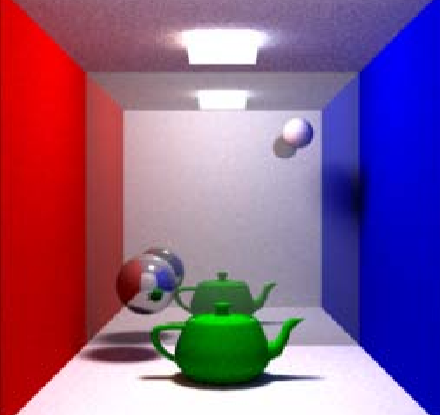
\includegraphics[width=.8\textwidth]{media/PathTracingMD.png}	
		\caption{\textit{Path Tracing} without noise.}
		\label{PT}
	\end{subfigure}
	\caption{Comparison \textit{Ray Tracing vs. Path Tracing}. Source: \citep[pp.~23--29]{Cassagnabere2004}}
\end{figure}

We can observe how the Path Tracing, in Figure \ref{RT}, produces soft shadows compared to Ray Tracing, Figure \ref{PT}. Also, we can see the noisy effect produced by the random sampling of Path Tracing if the number of samples is poor.

In that present project, we are going to create an application that implements the Path Tracing method trying to generate images that looks realistic. This application it's going to calculate each pixel of an image given some scene. There will be three versions. The first one is the sequential version, where one pixel is calculated at once and it's the base for all other versions. The other two versions are the CPU and GPU parallel versions. The reason to develop all of these versions is to be able to do a performance analysis about our algorithm both in GPU and CPU and decide which architecture is bringing more performance.

The implementation proposed by Peter Shirley in his books about Ray Tracing  \citep{ShirleyRTA, ShirleyRTB, ShirleyRTC} is going to be the base to develop our Path Tracer. The main intention is to develop three applications (sequential in CPU, parallel in CPU and GPU) to analyze how is the performance in both architectures CPU and GPU.

We will not only focus on the rendering section, although this is the central thread of this project, but we will also study which acceleration techniques are commonly used to try to improve our algorithm as much as possible. That is why we will also study which is the best way to represent internally the scene we want to render following the idea presented by \citep{Karras2012} in his paper.

The way we represent our scene will have a great impact on how we calculate the colour of the final image. As we have mentioned above, the basis of the method is to trace rays through the scene to calculate the colour of each pixel. If our representation of the scene consists of storing all the objects in a data structure such as a list or vector, ordered by order of creation, when calculating a point of the image in the worst case we will be going through the whole set of polygons of the scene to determine the final colour. Trying to render a scene that, very possibly, is composed of millions of polygons can translate into hours and hours of processing. That's why we'll make use of an accelerating data structure that allows us to represent the scene in a more clever way, so that when determining if a ray hits or not a polygon is determined in the fastest way possible.

\section{Justification}

As we have already pointed in the above section, we will start from the Peter Sherly books and Tero Karras paper about Bounding Volume Hierarchies. In this project, we expect to study how we can exploit at maximum the different architectures that we have in our computers (CPU and GPU) and decide how's more efficient. We cannot compare our application with an existing one. Because the professional applications that implement the Path Tracing algorithm are made by experts with plenty of experience and knowledge that will allow increasing the performance significantly, and the author of this project does not have. Moreover, in the field of realism, it's hard to compare because a professional application includes plenty of features such as subsurface scattering or tessellation. In this project, it's impossible to reach an application with similar characteristics. First of all, the lack of knowledge and experience in the field of realistic off-line rendering.
Finally, the time. Usually, a project with this scope involves plenty of specialists and need months or years to realise. A professional example of Path Tracer is RenderMan, developed by Pixar Animation Studios \citep{Christensen2018}.

For this reason, in this project, we will develop three versions of the same algorithm: \begin{enumerate*}[label=\roman*)] \item sequential version, \item parallel version in CPU and \item parallel version in GPU \end{enumerate*}. Therefore, we will analyze the versions with each other and decide the best architecture and version for our implementation.

Currently, there are plenty of libraries oriented to GPU programming. Libraries such as \texttt{OpenCL} and \texttt{OpenACC} provides us with portability between graphics cards from different manufacturers like \texttt{AMD} and \texttt{NVIDIA}. For this project, we decided to choose the CUDA environment developed by \texttt{NVIDIA}. \texttt{CUDA} is a parallel computing platform and API created for its graphics card and accelerators. The reason we chose this API is that being proprietary software it is more optimized for \texttt{NVIDIA} graphics cards, as indicated by \citep{Karimi2010} and \citep[pp.~216--215]{Fang2011} in their respective papers.

It is possible that citing the \texttt{NVIDIA} graphics cards and accelerators and, keeping in mind the project's focus on rendering realistic graphics, to the lector of this Final Degree Project comes to mind the new brand of RTX cards designed by \texttt{NVIDIA}. In the beginning, the idea was to orient the project to use RTX graphics cards because they have been designed specifically for the use of Ray Tracing in real-time. But, this idea was immediately rejected because of the high price of these. The price range varies between 350€ to 2000€ or 6000€ (for HPC). Finally, even the author of this project bought an RTX 2080 Super it was decided not to focus the project only in the new RTX technology. Exploring all the new features that these include such as RT Cores, Tensor Cores and Mesh Shaders would have meant starting the job all over again and losing a huge amount of time spent. Because it would have been necessary to learn all the necessary knowledge to develop the project. That does not imply that the graphics card should not be used. As a high-end graphics card, the number of cores it has compared to the GTX1050 (mid-range) will allow us to analyse how much better it is and whether or not it is worthwhile, in terms of cost/power ratio, to use it in applications of this type.

As we mentioned at the beginning of this section,  \texttt{CUDA} is an API very optimized for \texttt{NVIDIA} hardware. This gives us an advantage because all the environments that we will use in this project have NVIDIA technology

\begin{enumerate}
	\item Laptop - Lenovo Legion Y520 with an Nvidia GTX1050 Mobile - 4GB.
	\item Personal Computer - Nvidia RTX 2080 Super - 8Gb.
	\item Teaching cluster BOADA - 4 GPUs Nvidia Tesla K40c.
\end{enumerate}

The use of graphics cards in different environments will allow us to analyse how our application responds in each of them and thus study how performance is when we use several cards designed for a research/professional environment, as opposed to two others designed for more ordinary use. We will also be able to see how the performance is in a mid-range graphics card (Nvidia GTX1050 Mobile) and a high range one (Nvidia RTX 2080 Super) and make a comparison between them.

\section{Planning}

We can see in Figure \ref{gantt_esp}, Figure \ref{gantt_1} and Figure \ref{gantt_2} the first planning proposed for this project. But at the beginning of December, it was decided to postpone the delivery date to the April shift. The reason for this postponement is the change in the language of lecture and reporting. In the beginning, this project was conceived in Spanish, but we determined to change the language to English to certify competence in a foreign language.

Due to the extension of the project deadline, we decided to add more features to the project. In this case, we decided to add texturing and bilateral filtering to the resulting image. The parameters used for the bilateral filter will also be tested to find the best parametrization.

In Figure \ref{gantt_eng}, we can see the actual project planning and Figure \ref{gantt_4} shows the new stages added to the Main Development task. The other sub-stages from the Main Development task remain equals. The Final Stage is focused on the experiments and writing the final report as we can see in Figure \ref{gantt_4}.

\subsection{Gantt Chart}

\uselandscape

\begin{figure}[H]
	\centering
	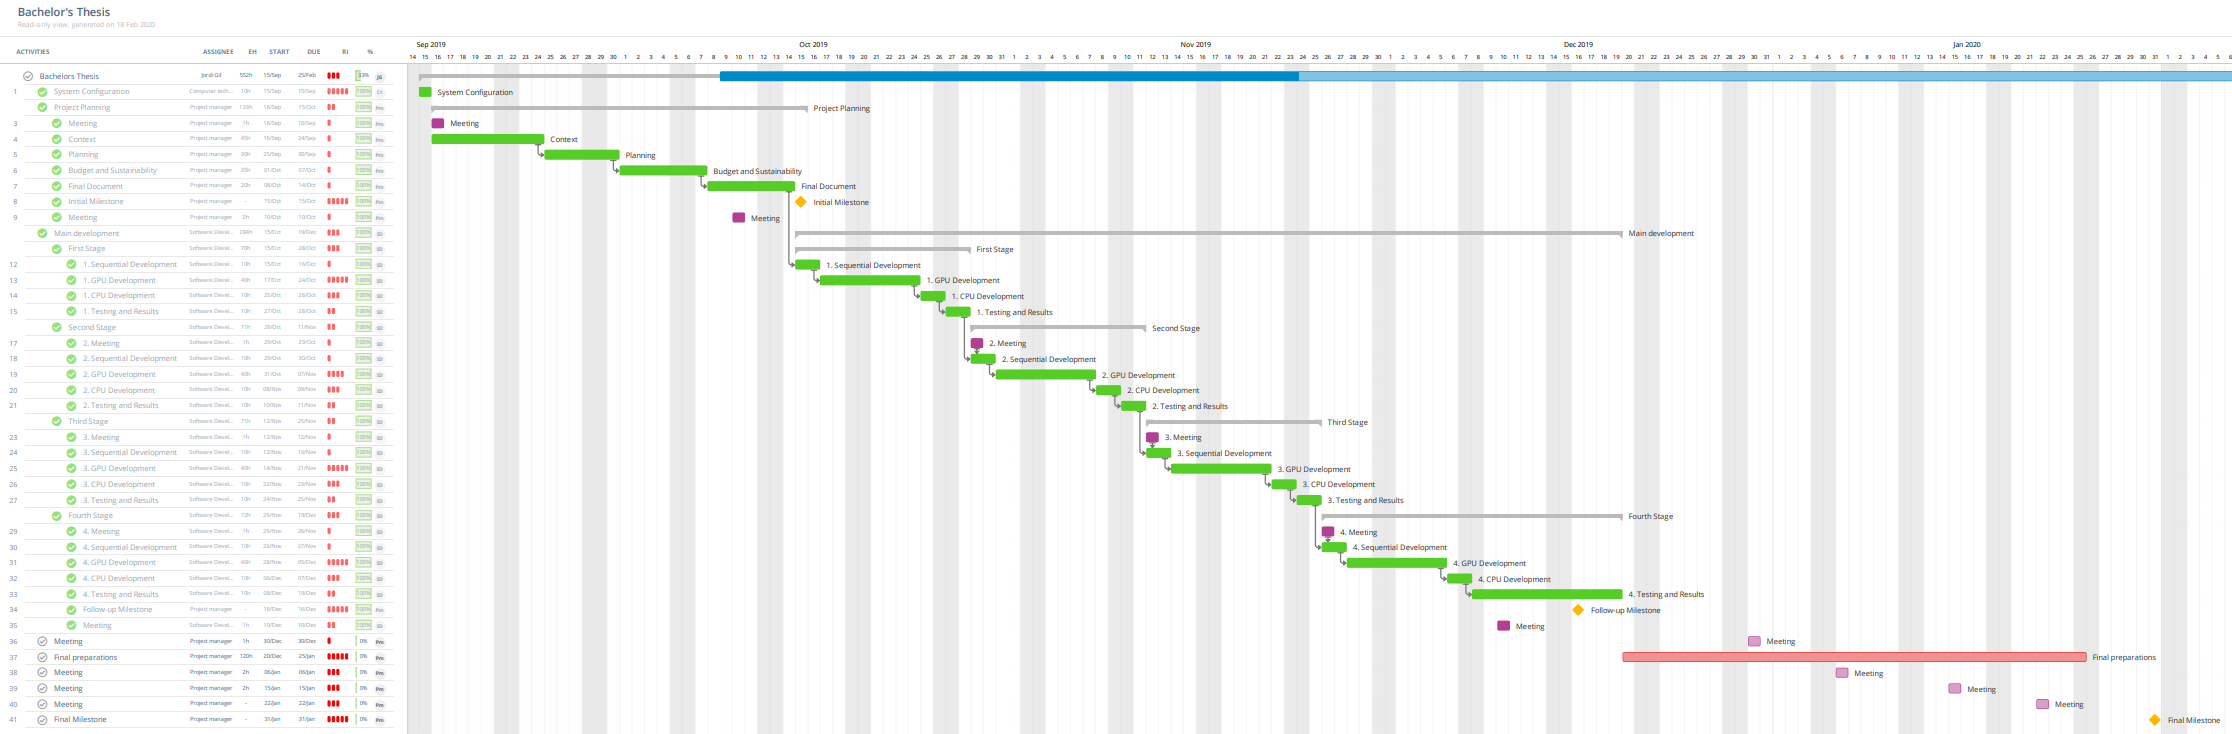
\includegraphics[scale=0.30]{media/final_gantt_esp.png}
	\captionof{figure}{Complete Gantt Chart.}
	\label{gantt_esp}
\end{figure}

\begin{figure}[H]
	\centering
  	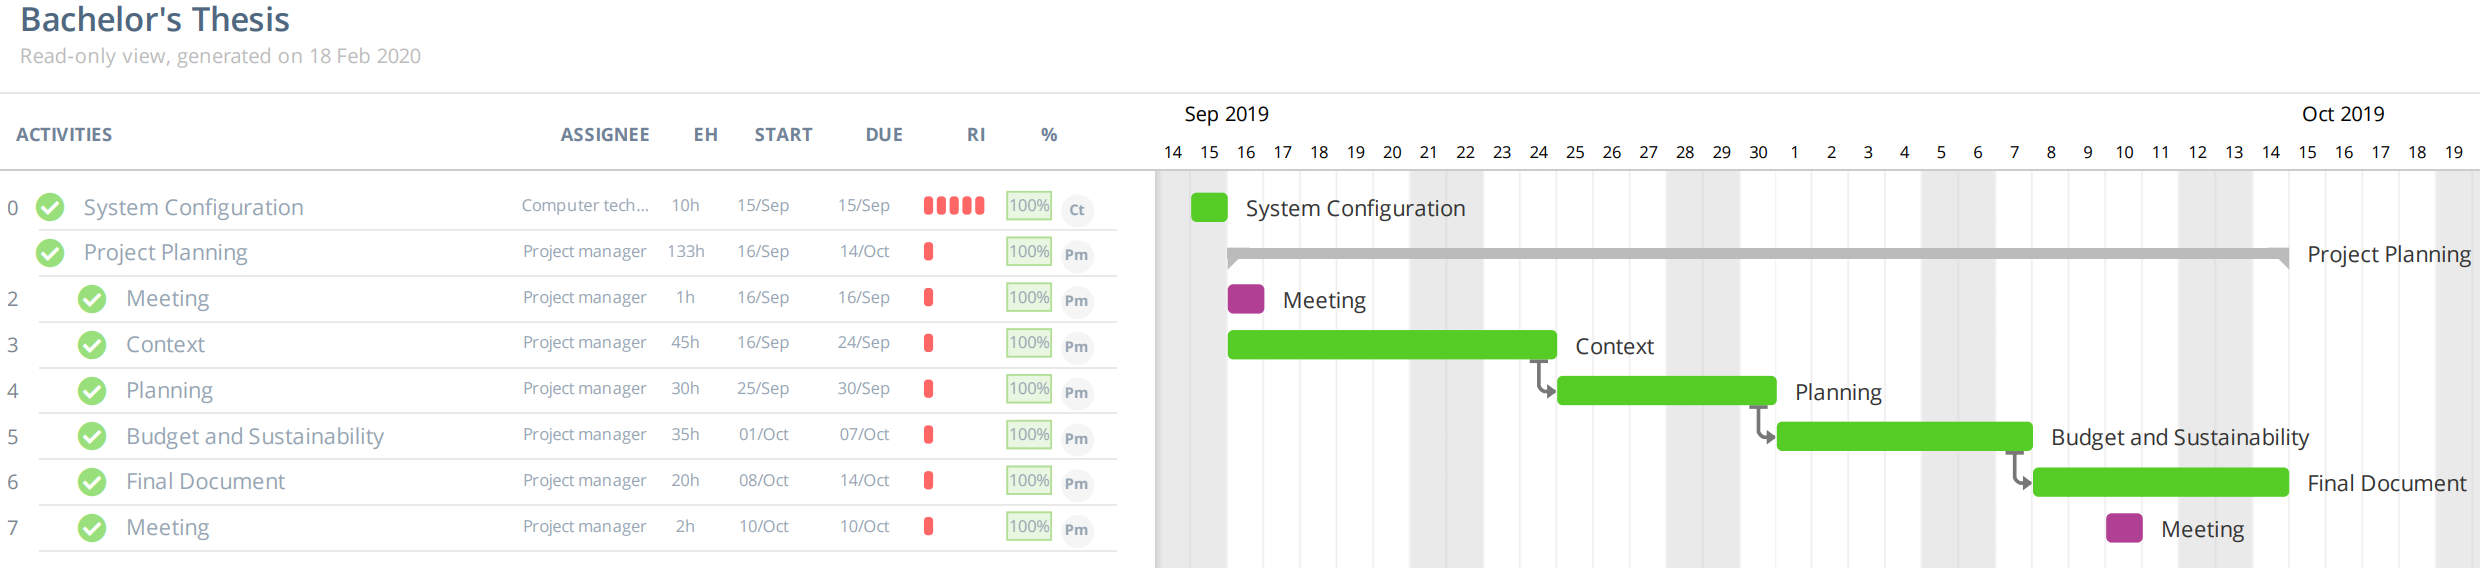
\includegraphics[scale=0.25]{media/gantt_gep.png}
  	\captionof{figure}{GEP Stage.}
  	\label{gantt_1}
\end{figure}

\begin{figure}[H]
	\centering
  	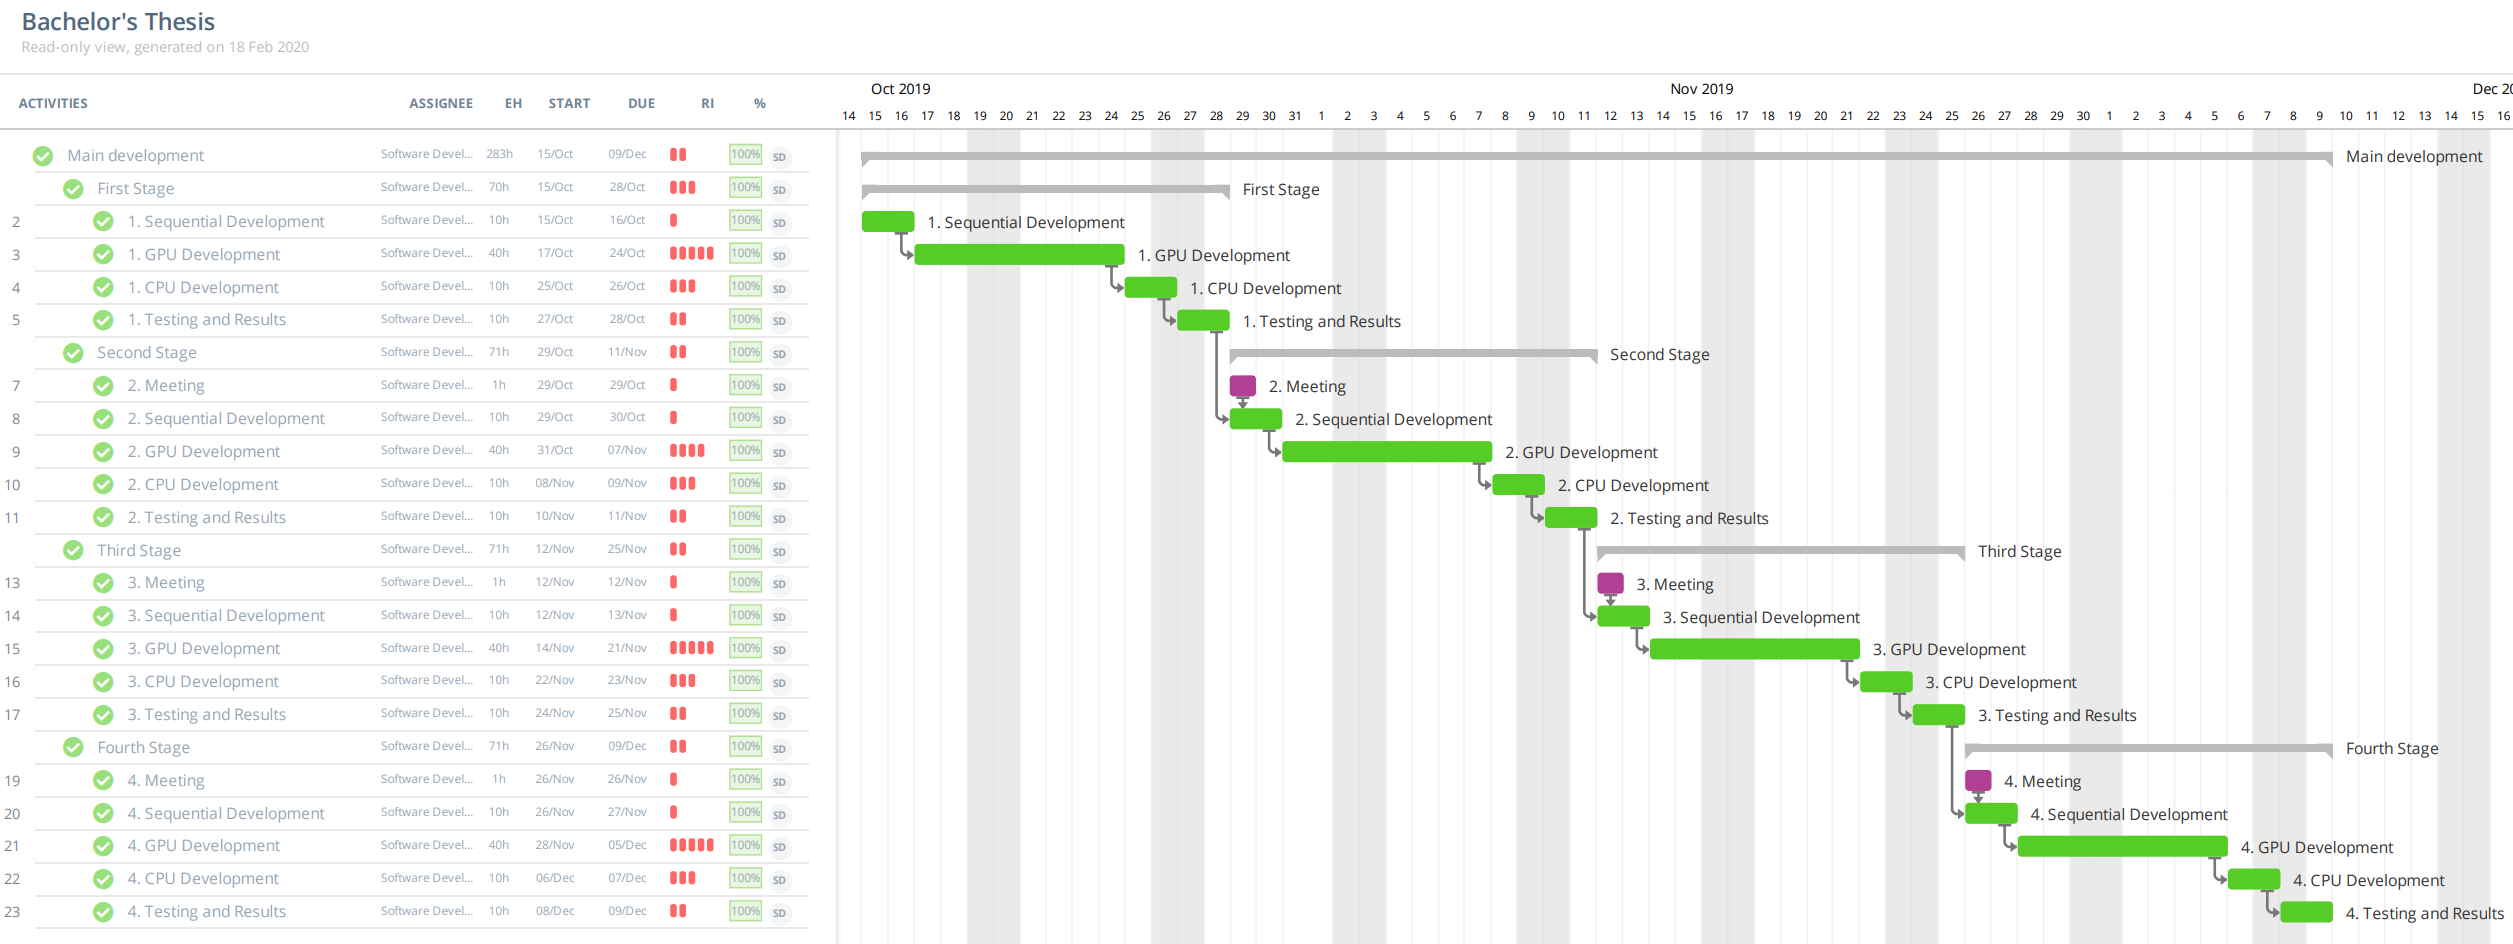
\includegraphics[scale=0.25]{media/gantt_dev_esp.png}
  	\captionof{figure}{Development Stage.}
  	\label{gantt_2}
\end{figure}

\begin{figure}[H]
	\centering
	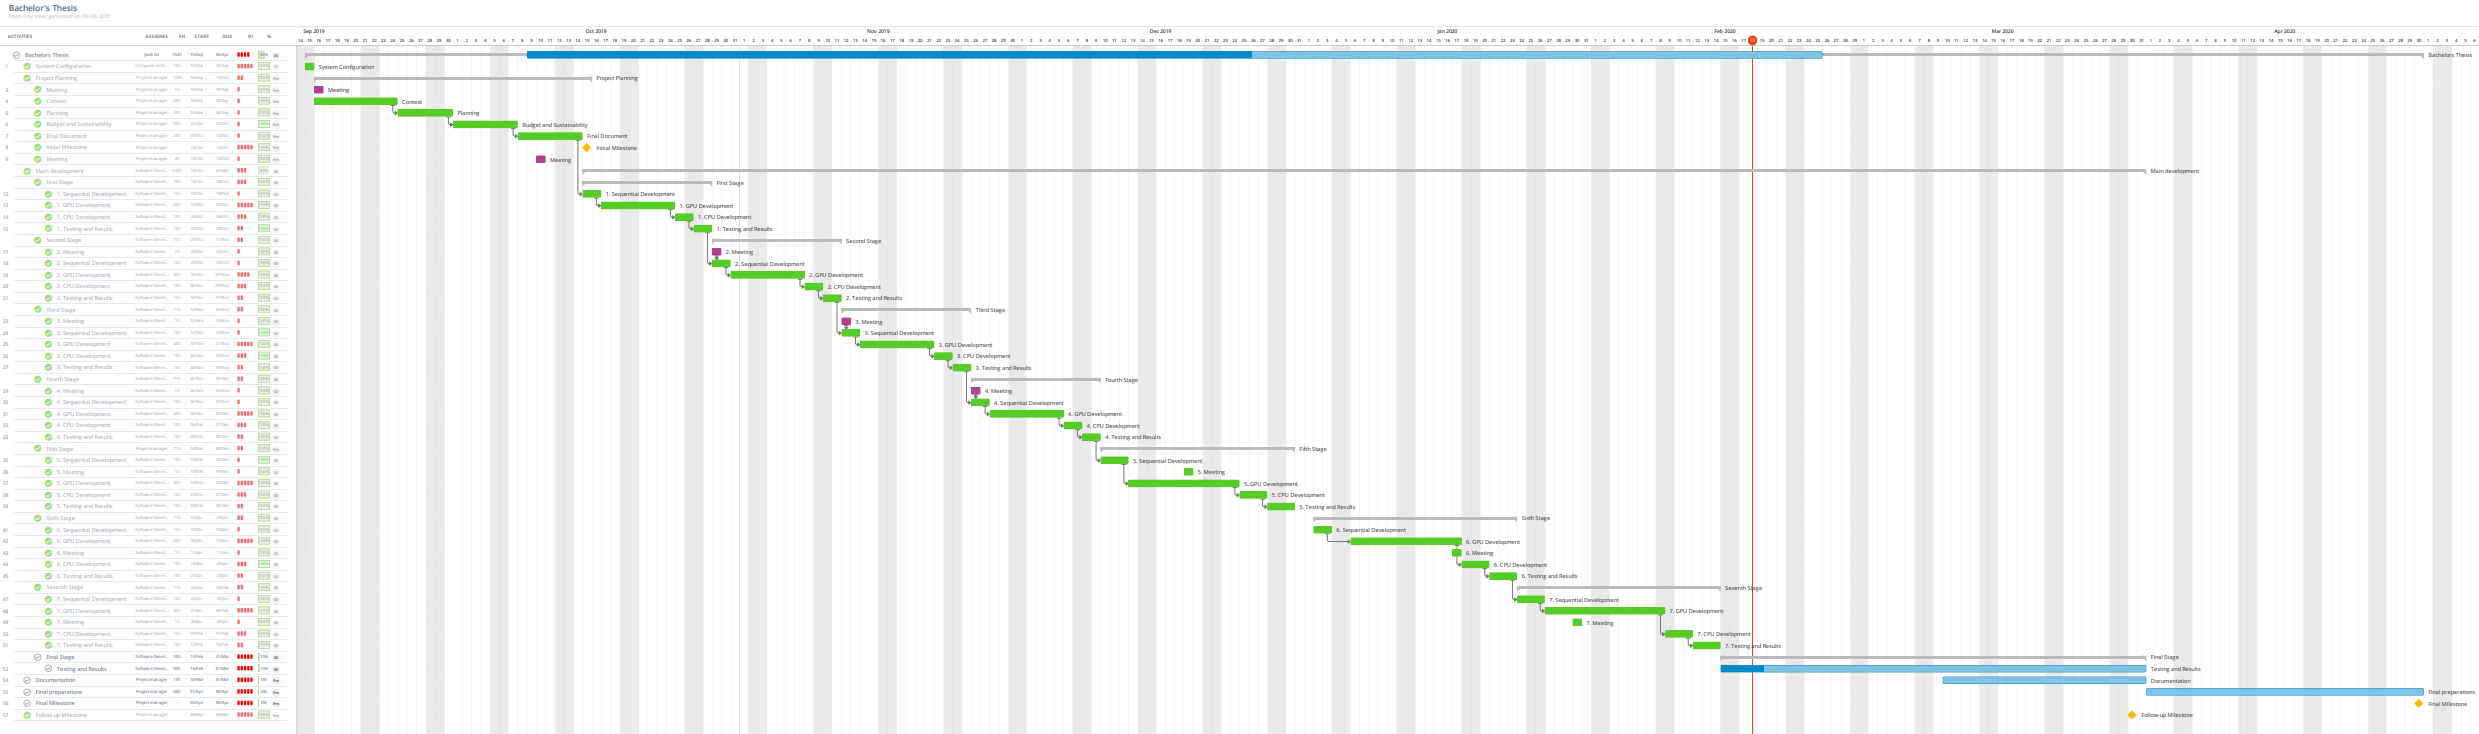
\includegraphics[scale=0.30]{media/final_gantt_eng.png}
	\captionof{figure}{Complete Gantt Chart.}
	\label{gantt_eng}
\end{figure}

\begin{figure}[H]
	\centering
  	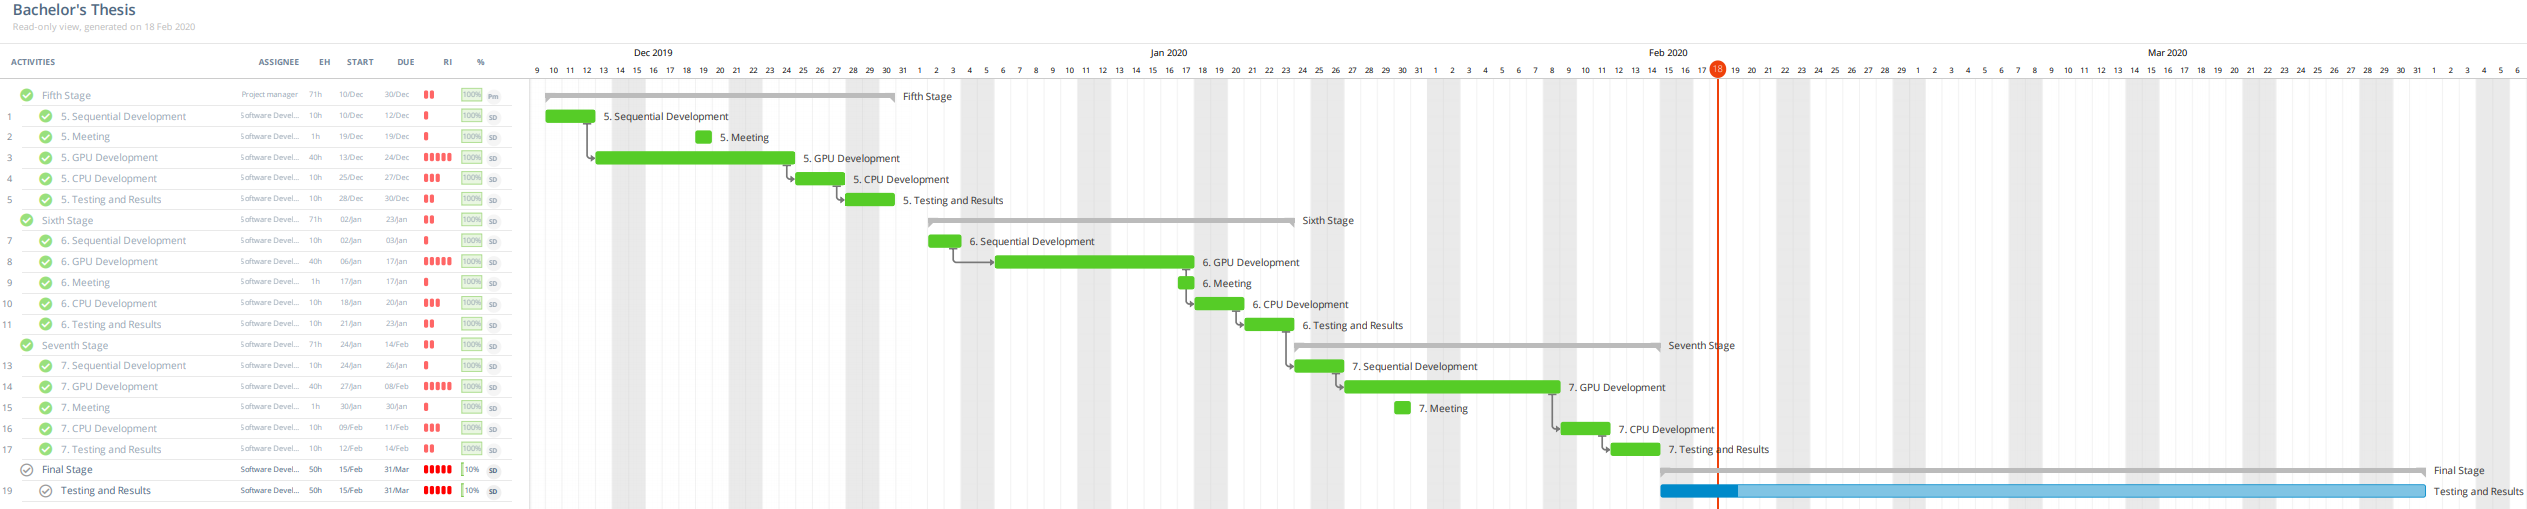
\includegraphics[scale=0.25]{media/gantt_dev_eng_new.png}
  	\captionof{figure}{Development Stage new tasks.}
  	\label{gantt_3}
\end{figure}

\begin{figure}[H]
	\centering
  	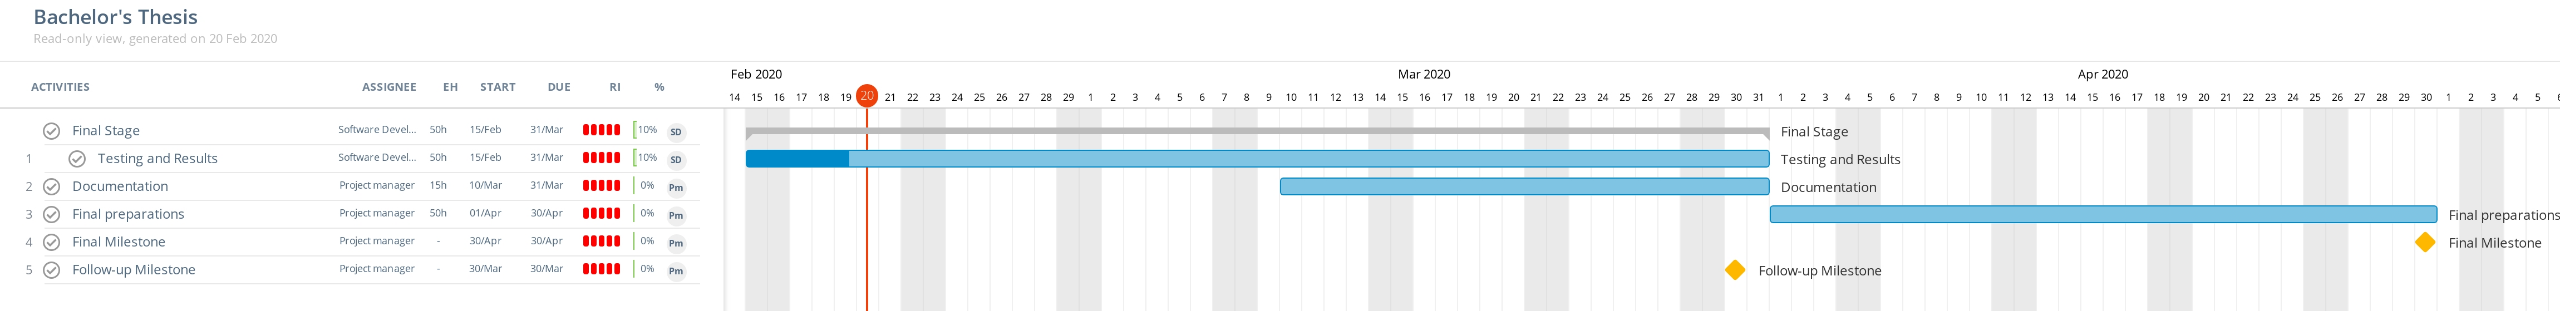
\includegraphics[scale=0.25]{media/gantt_final_eng.png}
  	\captionof{figure}{Final Stage.}
  	\label{gantt_4}
\end{figure}

\useportrait

\section{Methodology}

The methodology followed is the same as we established at the start of the project. This methodology has allowed us to develop the project in stages so that we can have an overview of the project status.

\section{Alternative Analysis}

During the project planning the main objectives were clearly and concisely defined, and this has allowed us to know in all moments which goals have been reached and have not.

Besides, in the case of not being able to provide different shapes to represent our 3D models such as spheres or triangles, we will only use triangles because of the versatility that these give us.

\section{Knowledge Integration}

Principally, the knowledge integrated into the project corresponds to the knowledge acquired in the Computer Science speciality, as well as some obligatory subjects of the degree and optional ones. The familiarity about realistic rendering and application of geometric transforms on 3D objects, discussed in the subject of graphics, has been required. Also, the topics studied in subjects such as Parallelism and TGA, have been very important to develop our parallel applications.

Having knowledge in programming in languages like \texttt{C} or \texttt{C++} has been important for the proper development of the project.

\section{Identification of laws and regulations}

As we said in the first delivery, the main objective of the project is to allow the author to enter the field of computer rendering, in particular realistic rendering. For this reason, there are no laws or regulations that can be applied because it is not intended to make a commercial product. Furthermore, all the material and tools used during the project are for free use or self-created.


\newpage

\printbibliography

\listoffigures

\listoftables

\end{document}
